\documentclass[tikz,border=10pt]{standalone}
\begin{document}
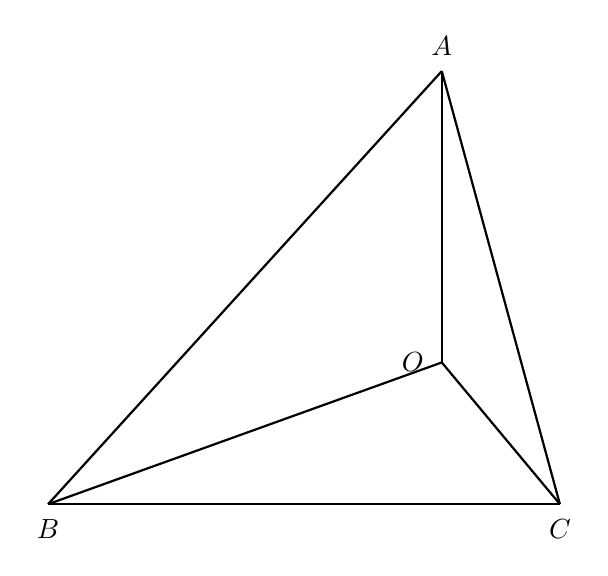
\begin{tikzpicture}
\coordinate (A) at (5,5.5);
\coordinate (B) at (0,0);
\coordinate (C) at (6.5,0);
\coordinate (O) at (5,1.8);

\draw[thick] (A) -- (B);
\draw[thick] (A) -- (C);
\draw[thick] (B) -- (C);
\draw[thick] (A) -- (O);
\draw[thick] (B) -- (O);
\draw[thick] (C) -- (O);

\node[above=2pt] at (A) {$A$};
\node[below=2pt] at (B) {$B$};
\node[below=2pt] at (C) {$C$};
\node[left=3pt] at (O) {$O$};
\end{tikzpicture}
\end{document}
